\subsubsection{Software}
\textbf{Åbningscontrolleren} er designet på baggrund af systemarkitekturen og de overvejelser, der hidtil har forløbet sig gennem sektion \ref{sec:Design}. \\
\textbf{Åbningscontrolleren} skal kunne styre en motor, som står for iskruning i proppen, og en motor, som står for at trække proppen ud. Ydermere skal den modtage kommandoer fra og give statusmeddelelser tilbage til \textbf{Positionscontrolleren}. \\
\\
Følgende kan der opstilles 3 grænsefladeklasser for \textbf{Åbningscontrolleren}: \\
\\
\textbf{PSoC\_SPI}, hvorigennem kommunikationen med \textbf{Positioneringscontrolleren} foregår. \\
\textbf{MotorS}, som styrer motoren for skruen. \\
\textbf{MotorP}, som styrer motoren for proptrækkeren. \\

\myparagraph{Sekvensdiagram}
Sekvensdiagrammet i figur \ref{sd:Aab} viser, hvordan der kommunikeres mellem klasserne, og hvilken overordnet funktionalitet, disse indeholder. Det skal dog understreges, at, dersom der ikke er et færdigt hardware-design af \textbf{Åbningsmekanismen}, er følgende diagram og funktionsbeskrivelser kun et bud på et muligt software-design.

\begin{figure}[H]
	\centerline{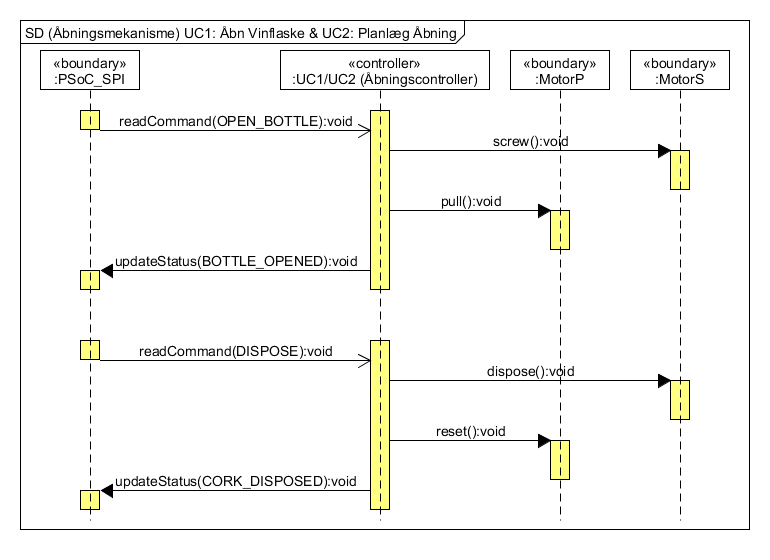
\includegraphics[scale=0.33]{tex/Design/PSoC/Diagrammer/SD_Aabningsmekanisme}}
	\caption{Sekvensdiagram over \textbf{Åbningsmekanisme}}
	\label{sd:Aab}
\end{figure}

\noindent Åbningen af vinflasken påbegyndes efter ordre fra \textbf{Positionsmekanismen}. Iskruning påbegyndes, og der skrues i proppen indtil skruen har fat i denne, hvorefter proppen trækkes ud. Herefter meddeles om dette til \textbf{Positionscontrolleren}, og efter ordre dispenseres proppen, og der meddeles om dette. \\

\myparagraph{Funktionsbeskrivelse}
Metoderne kan kort beskrives:

\textbf{screw()} skal sætte skruen til at dreje et forudbestemt antal steps.

\textbf{pull()} skal få proptræksmotoren til hive i proppen, indtil en trykknap rammes.

\textbf{dispose()} skal blot dreje skruen et vis antal steps for at disponere proppen.

\textbf{reset()} kører proptræksmotoren trykknap ved startpositionen er påtrykt.